\documentclass[aspectratio=169, 11pt]{beamer}

\usetheme{metropolis}
\usepackage{appendixnumberbeamer}

\usecolortheme[snowy]{owl}

\usepackage{booktabs}
\usepackage[scale=2]{ccicons}

\usepackage{pgfplots}
\usepgfplotslibrary{dateplot}

\usepackage{xspace}
\newcommand{\themename}{\textbf{\textsc{metropolis}}\xspace}



\title{ImageNet Classification with Deep Convolutional
Neural Networks}
\author{Sidharth S}
\subtitle{Seminar}
\date{\today}

\institute{Rajagiri School of Engineering and Technology}
% \titlegraphic{\hfill\includegraphics[height=1.5cm]{logo.pdf}}

\begin{document}

\maketitle % prints title
\metroset{block=fill, titleformat=smallcaps}

%Slide 1

\begin{frame}
\frametitle{Introduction}
\begin{itemize}
\item AlexNet
\item One of the most influential papers published in computer vision.
	\begin{itemize}
	\item  AlexNet paper has been cited over 70,000 times according to Google Scholar.
	\end{itemize}
\item The network achieved a top-5 error of 15.3\%.
\item It is the first CNN where multiple convolution operations were used.
\end{itemize}

\begin{figure}
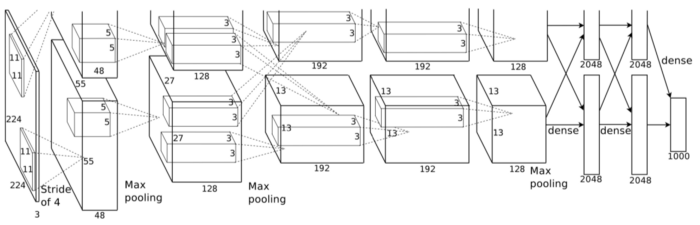
\includegraphics[scale=0.4]{alexnet}
%\centering \
\caption{AlexNet Architecture}
%\vspace{3pt}
\end{figure}

\end{frame}

%Slide 2
\begin{frame}
	\frametitle{Abstract}
	\begin{itemize}
		\item Deep convolutional neural network to classify the 1.2 million
high-resolution image.
		\item 60 million parameters and 650,000 neurons.
		\item Convolutional Layers, Maxpooling layers, Fully connected layers and Softmax
		\item GPU implementation of the convolution operation.
		\item Dropout regularization.
	\end{itemize}

\end{frame}

%Slide3
\begin{frame}
	\frametitle{Problem With Fully Connected Networks}
	\begin{block}{Fully Connected Neural Networks}
	\emph{Fully connected neural networks (FCNNs)} are a type of neural network where the architecture is such that all the nodes, or neurones, in one layer are connected to the neurones in the next layer. 
	\end{block}
	For a $64 x 64 x 3$ image,\\
	No of parameters in input layer = $12,288$
	\\
	\vspace{4pt}
	For a $225x225x3$ image,\\
	No of parameters in input layer = $151,875$
	\begin{itemize}
		\item Networks having large number of parameter face several problems, for 				e.g. slower training time, chances of overfitting e.t.c.
	\end{itemize}

\end{frame}

%Slide 4

\begin{frame}
	\frametitle{Convulutional Neural Networks (CNN)}

	\begin{block}{Convolution}
		In mathematics, \alert{convolution} is a mathematical operation on two 					functions $f$ and $g$ that produces a third function $f * g$ that expresses 			how the shape of one is modified by the other.
	\end{block}
 	
	\begin{itemize}
		\item The main image matrix is reduced to a matrix of lower dimension in the first layer itself
		\item  The role of the ConvNet is to reduce the images into a form which is easier to process, without losing features which are critical for getting a good prediction.
	\end{itemize}
		
\end{frame}

%Slide 5
\begin{frame}
	\frametitle{How Convolution is performed}
	We can use an input image and a filter to produce an output image by convolving the filter with the input image.\\
	\vspace{5pt}
	\textbf{Steps:}
	\begin{enumerate}
		\item Overlaying the filter on top of the image at some location.
		\item Performing \textbf{element-wise multiplication} between the values in the filter and their corresponding values in the image.
		\item Summing up all the element-wise products. This sum is the output value for the destination pixel in the output image.
		\item Repeating for all locations.
	\end{enumerate}




\end{frame}

\end{document}